%!TEX root = ../thesis.tex
% ******************************* Thesis Appendix D ********************************

\chapter{dL/dx vs. dE/dx plots} \label{appendixD:dldxVsDedxPlots}

\begin{figure}[htbp]
 \centering
 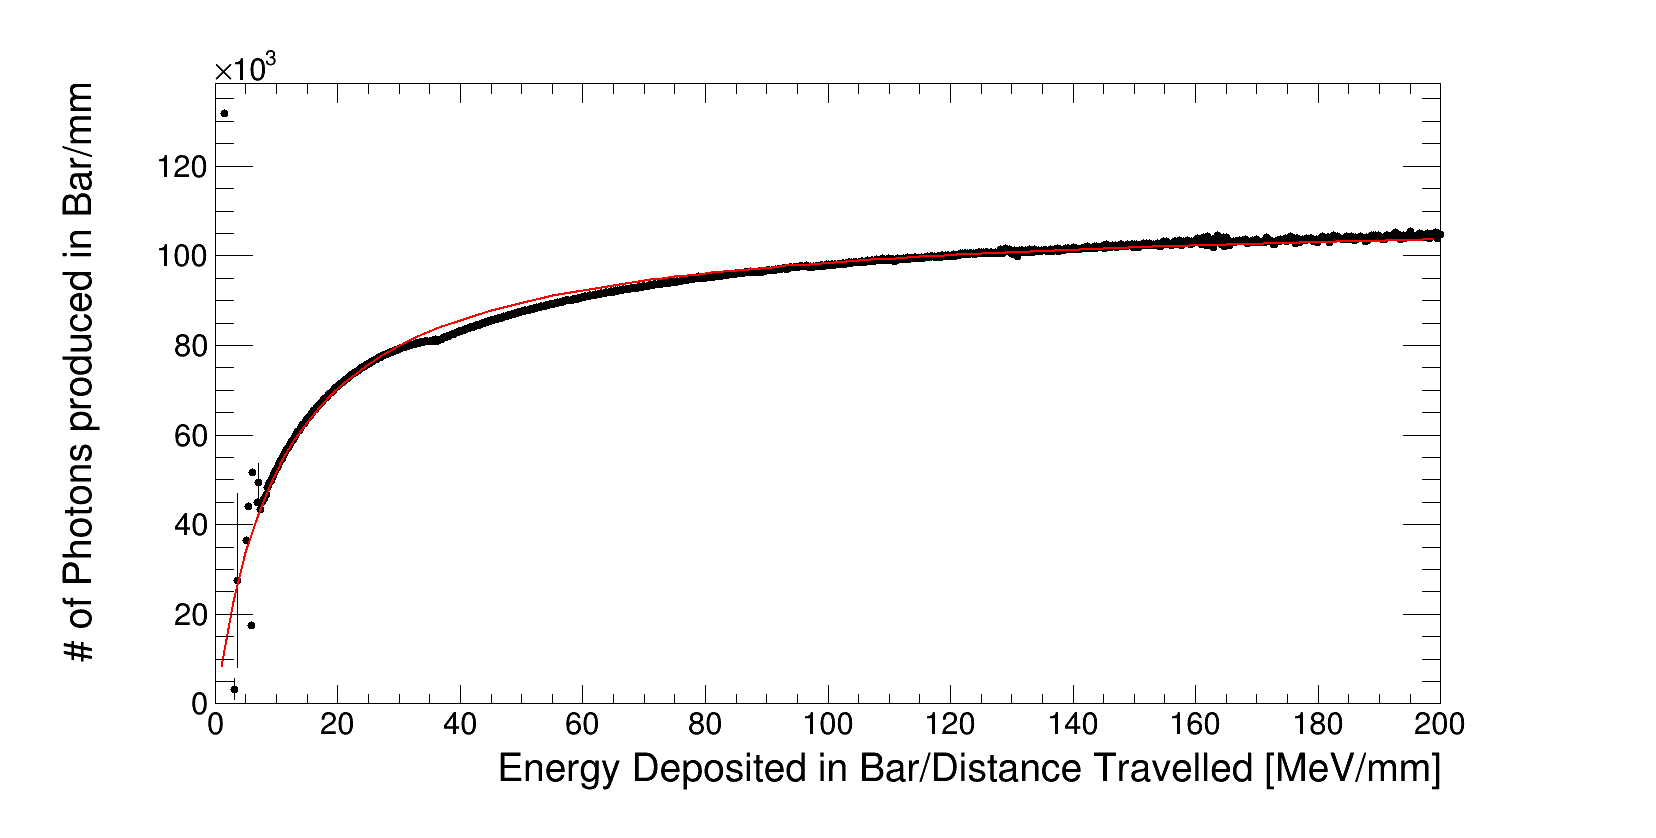
\includegraphics[width=\linewidth]{Appendix4/Figs/newDldxVsDedx/alpha_deDx_vs_dlDx.png}
 \captionof{figure}{dL/dx vs dE/dx fit using the approximation $\Delta L$/$\Delta x$ vs $\Delta E$/$\Delta x$ from the ``slice model'' simulation of scintillator for 1E6 simulated $\alpha$ particles, $\chi^2$ = 7466.2.} 
 \label{fig:slice_Alpha_dl_dx} 
\end{figure}

\begin{figure}[htbp]
 \centering
 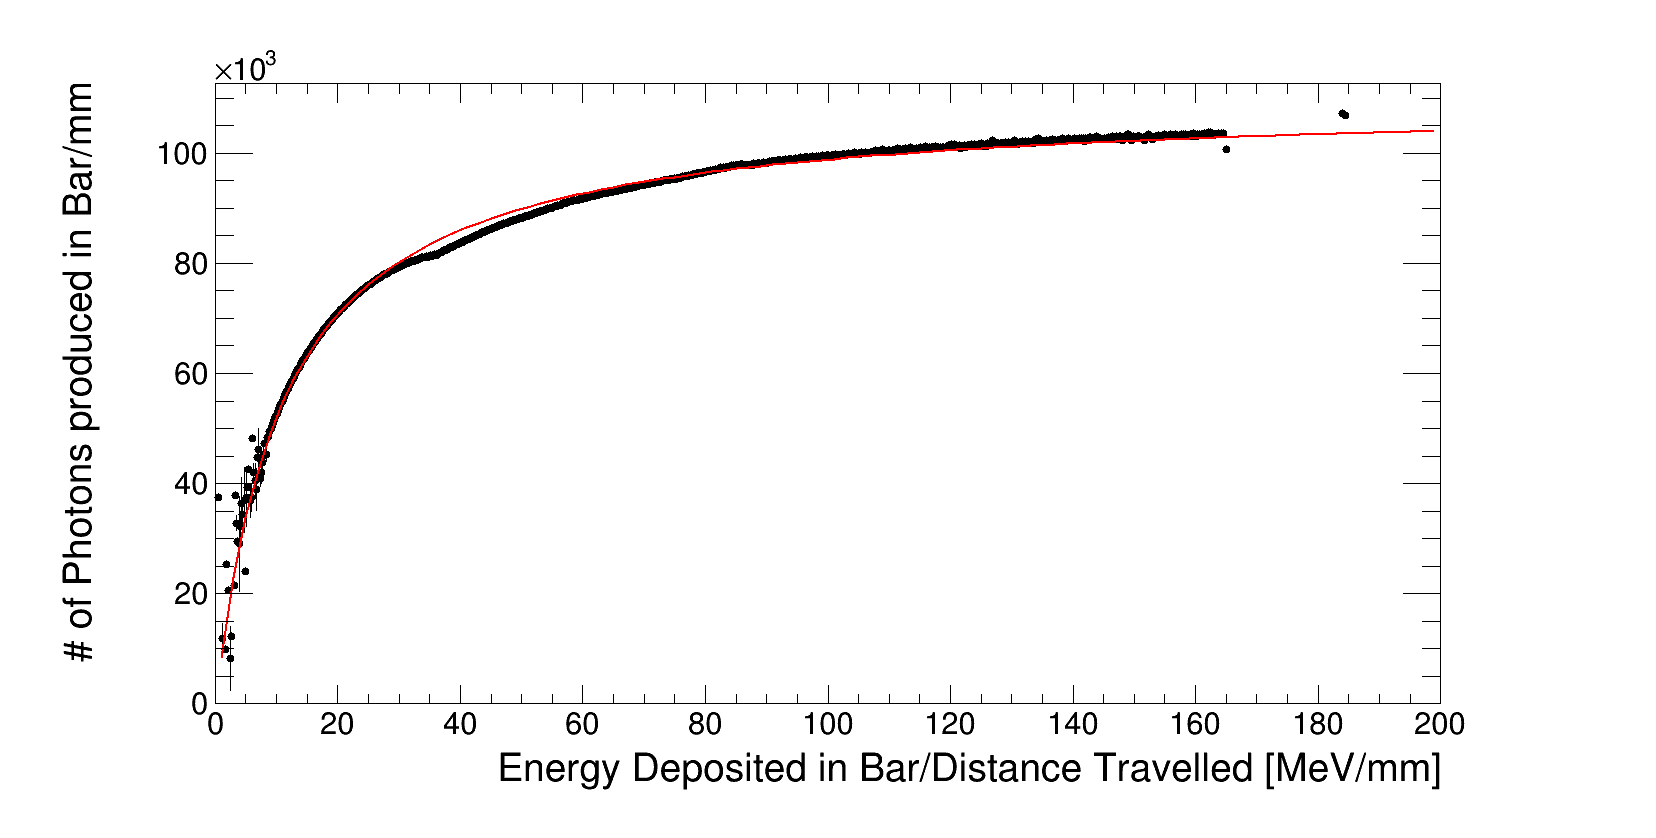
\includegraphics[width=\linewidth]{Appendix4/Figs/newDldxVsDedx/antiAlpha_deDx_vs_dlDx.png}
 \captionof{figure}{dL/dx vs dE/dx fit using the approximation $\Delta L$/$\Delta x$ vs $\Delta E$/$\Delta x$ from the ``slice model'' simulation of scintillator for 1E6 simulated $\Bar{\alpha}$ particles, $\chi^2$ = 4304.84.} 
 \label{fig:slice_AAlpha_dl_dx}
\end{figure}

\begin{figure}[htbp]
 \centering
 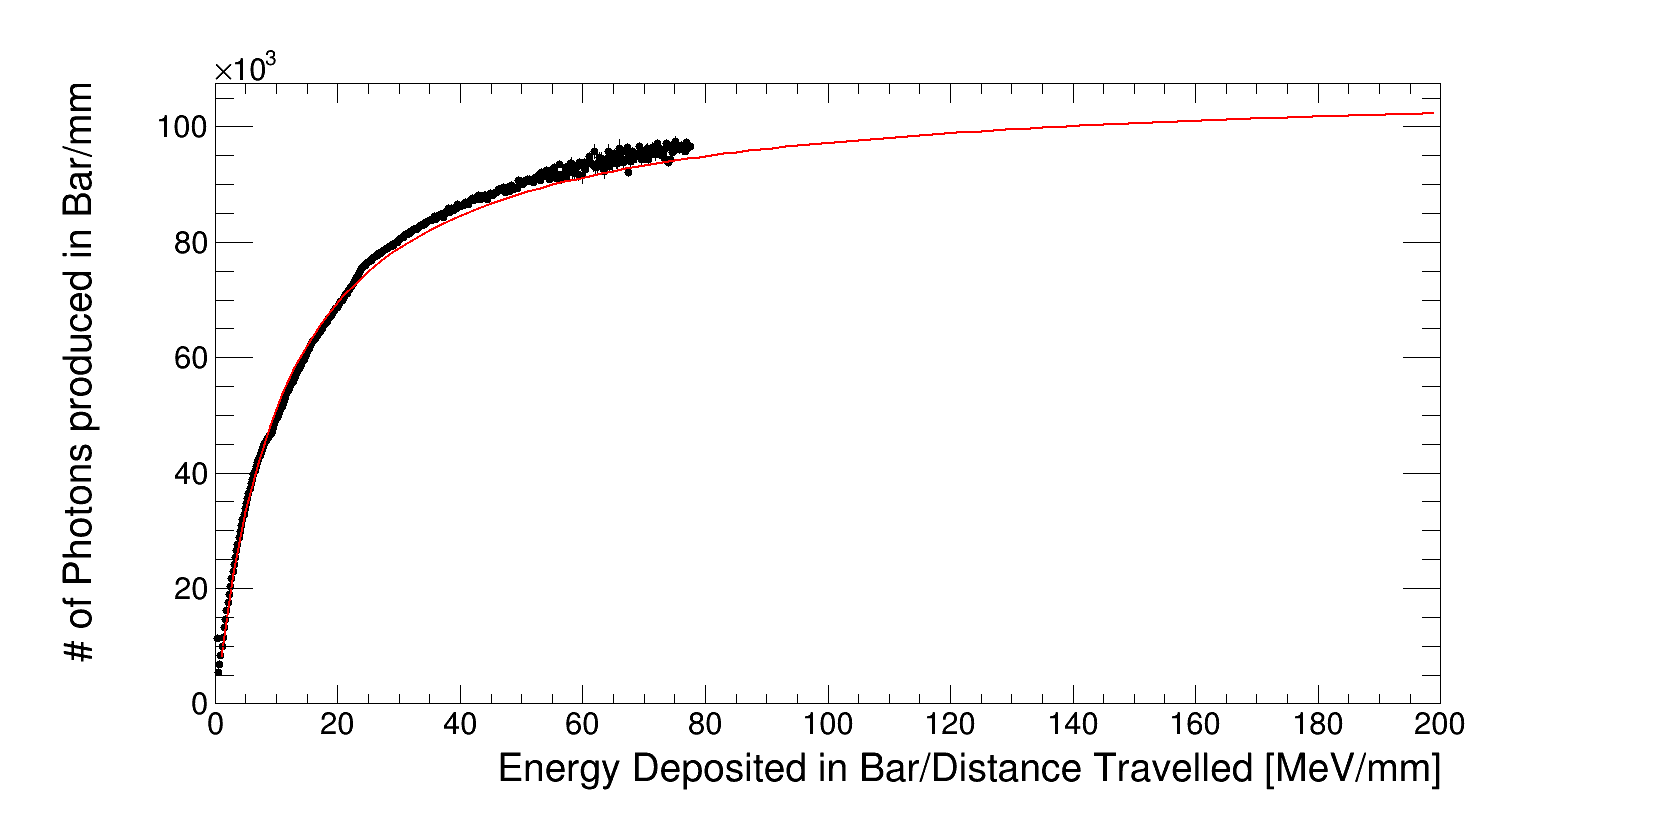
\includegraphics[width=\linewidth]{Appendix4/Figs/newDldxVsDedx/proton_deDx_vs_dlDx.png}
 \captionof{figure}{dL/dx vs dE/dx fit using the approximation $\Delta L$/$\Delta x$ vs $\Delta E$/$\Delta x$ from the ``slice model'' simulation of scintillator for 1E6 simulated proton particles, $\chi^2$ = 3734.22.} 
 \label{fig:slice_Proton_dl_dx}
\end{figure}

\begin{figure}[htbp]
 \centering
 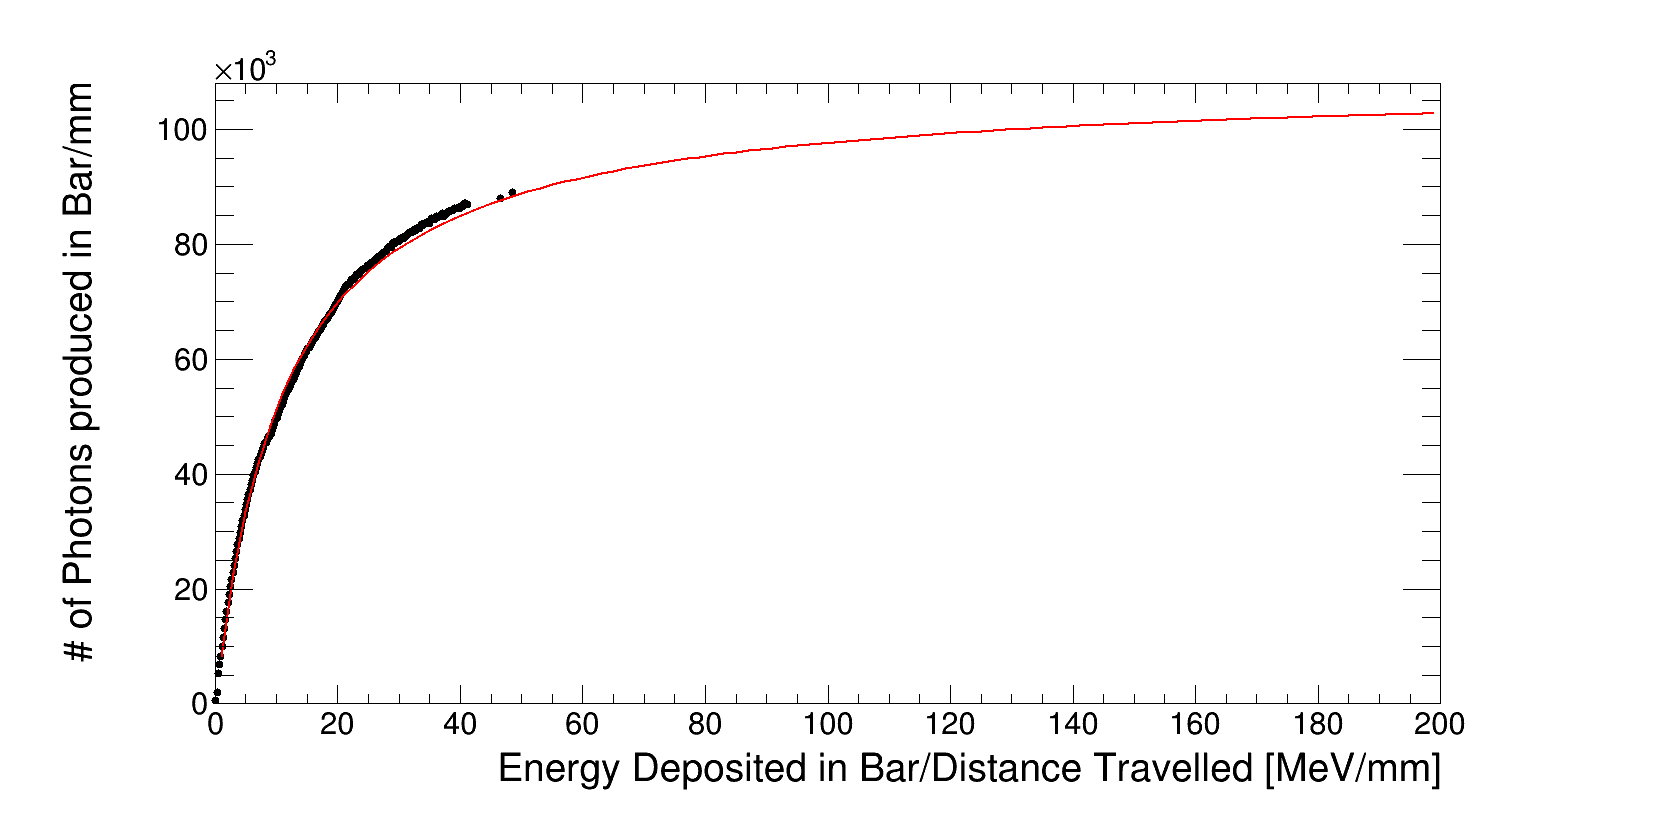
\includegraphics[width=\linewidth]{Appendix4/Figs/newDldxVsDedx/antiProton_deDx_vs_dlDx.png}
 \captionof{figure}{dL/dx vs dE/dx fit using the approximation $\Delta L$/$\Delta x$ vs $\Delta E$/$\Delta x$ from the ``slice model'' simulation of scintillator for 1E6 simulated anti-proton particles, $\chi^2$ = 5065.57.} 
 \label{fig:slice_AProton_dl_dx}
\end{figure}

\begin{figure}[htbp]
 \centering
 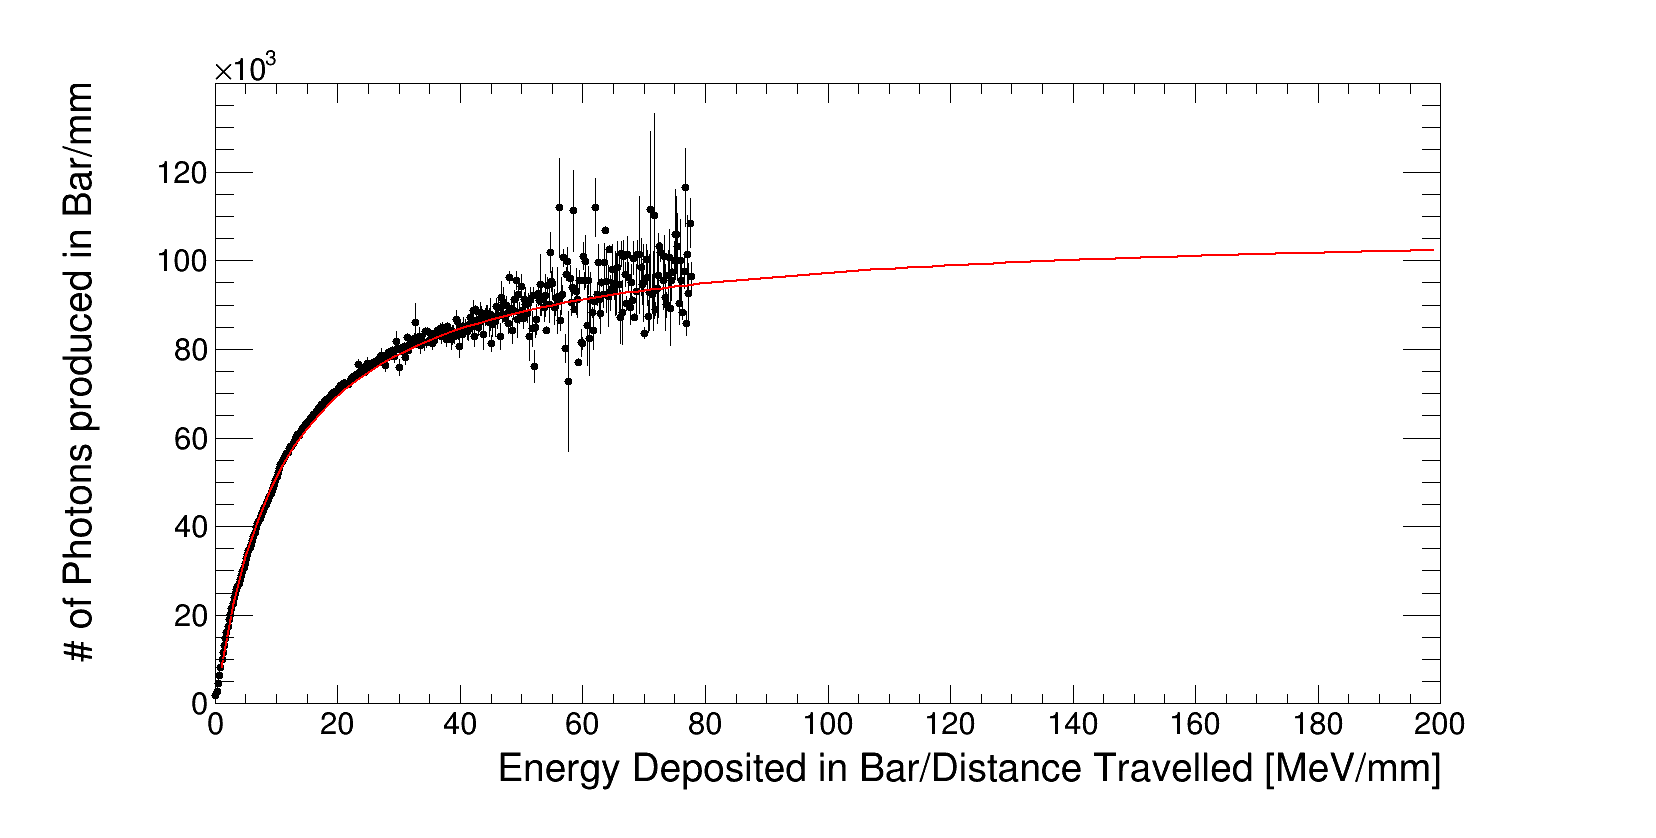
\includegraphics[width=\linewidth]{Appendix4/Figs/newDldxVsDedx/pi+_deDx_vs_dlDx.png}
 \captionof{figure}{dL/dx vs dE/dx fit using the approximation $\Delta L$/$\Delta x$ vs $\Delta E$/$\Delta x$ from the ``slice model'' simulation of scintillator for 1E6 simulated $\pi^+$ particles, $\chi^2$ = 13966.8.} 
 \label{fig:slice_APiPlus_dl_dx}
\end{figure}

\begin{figure}[htbp]
 \centering
 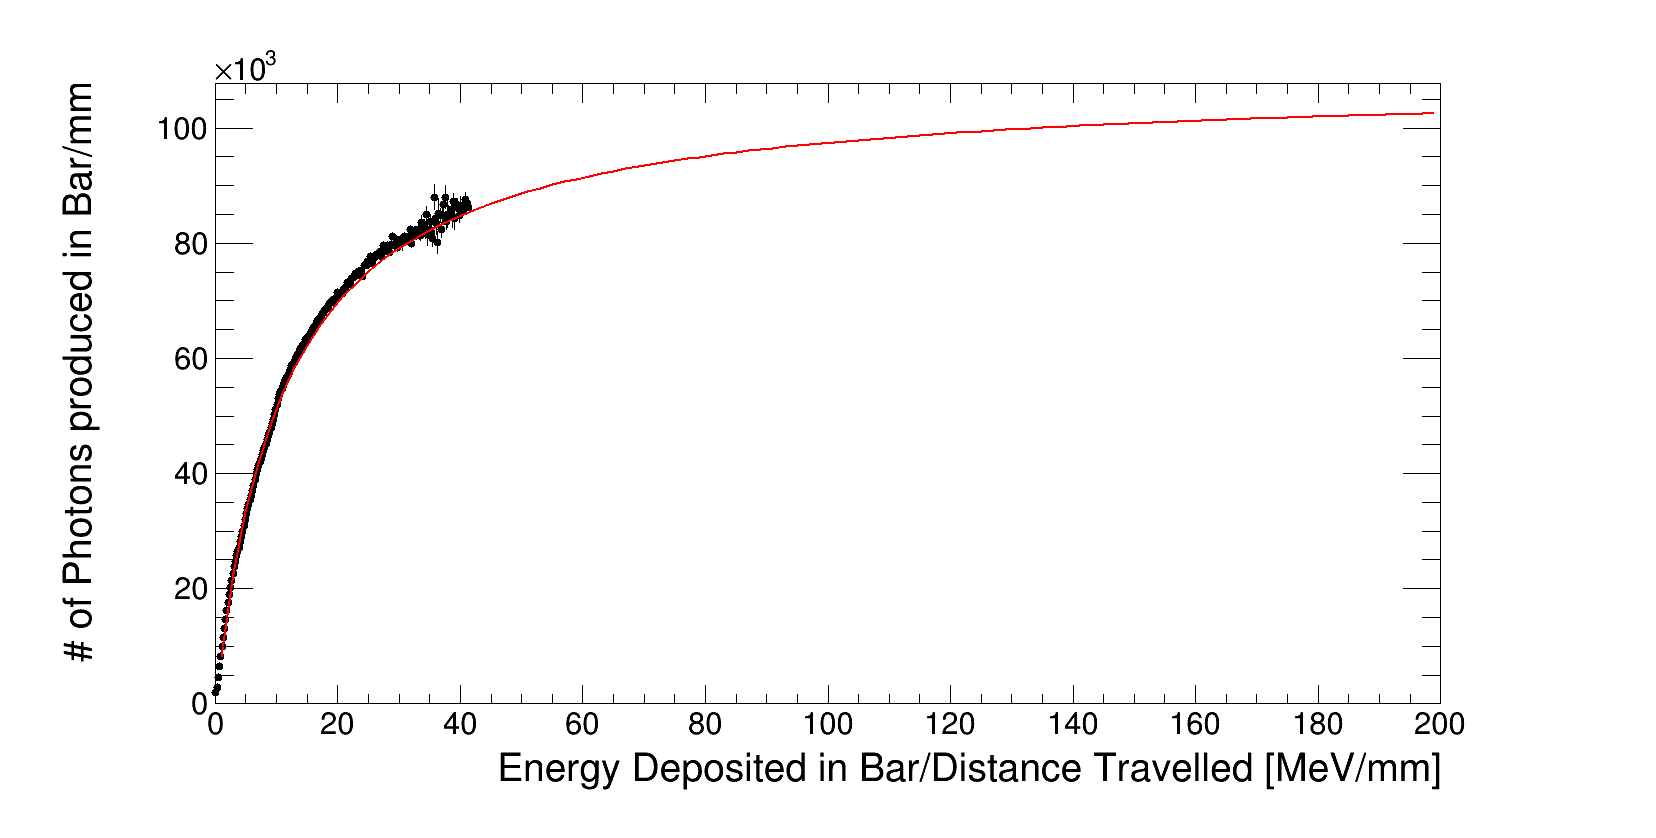
\includegraphics[width=\linewidth]{Appendix4/Figs/newDldxVsDedx/pi-_deDx_vs_dlDx.png}
 \captionof{figure}{dL/dx vs dE/dx fit using the approximation $\Delta L$/$\Delta x$ vs $\Delta E$/$\Delta x$ from the ``slice model'' simulation of scintillator for 1E6 simulated $\pi^-$ particles, $\chi^2$ = 25852.4.} 
 \label{fig:slice_APiMinus_dl_dx}
\end{figure}

\begin{figure}[htbp]
 \centering
 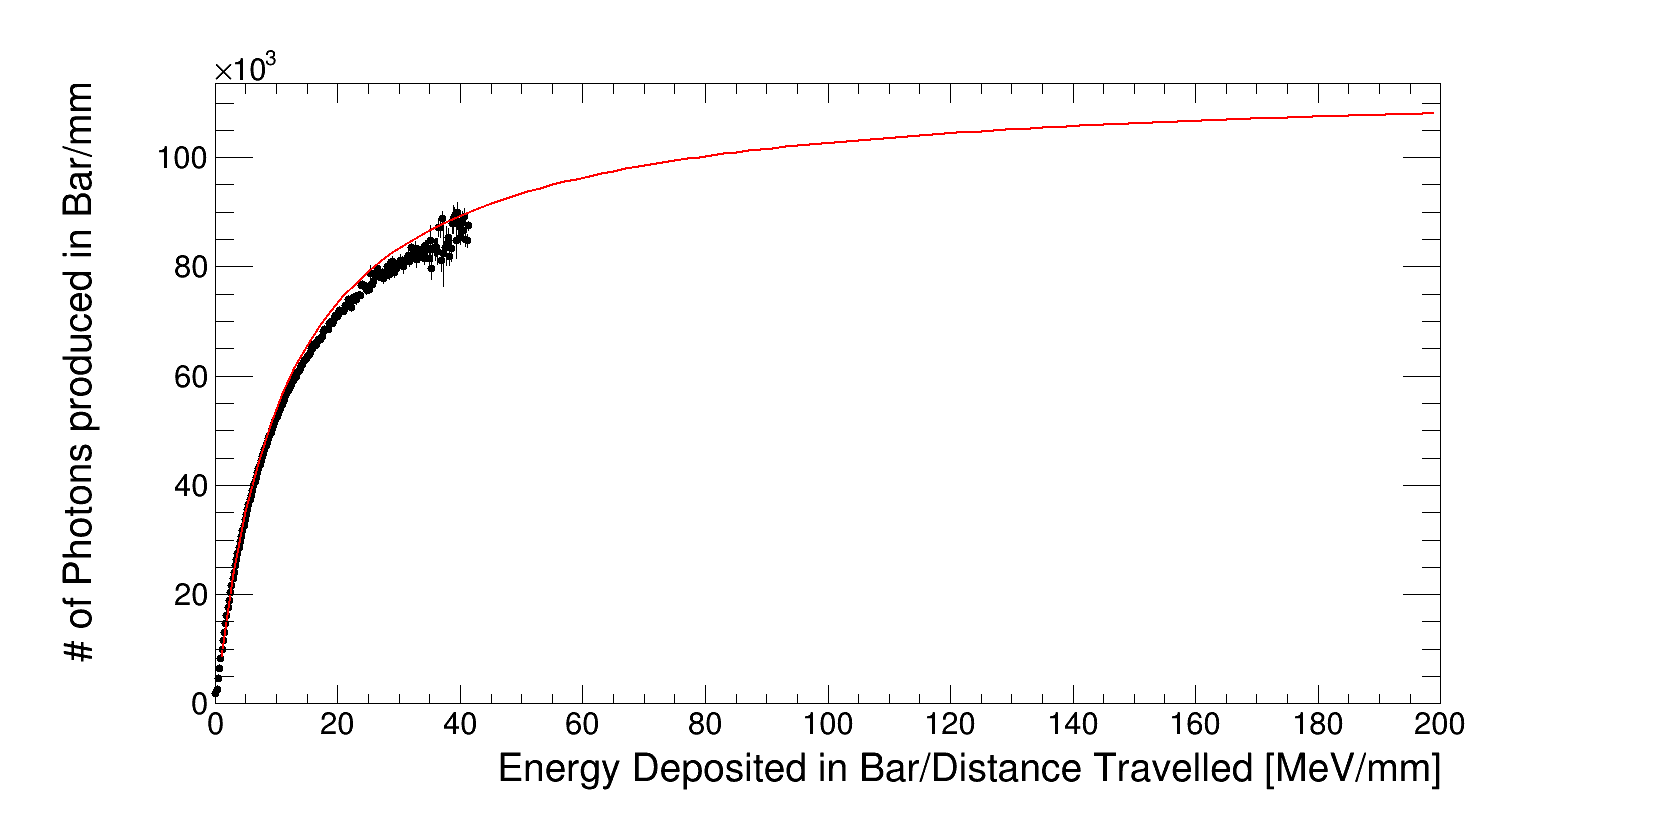
\includegraphics[width=\linewidth]{Appendix4/Figs/newDldxVsDedx/mu-_deDx_vs_dlDx.png}
 \captionof{figure}{dL/dx vs dE/dx fit using the approximation $\Delta L$/$\Delta x$ vs $\Delta E$/$\Delta x$ from the ``slice model'' simulation of scintillator for 1E6 simulated $\mu^-$ particles, $\chi^2$ = 46098.1.} 
 \label{fig:slice_Muon_dl_dx}
\end{figure}

\begin{figure}[htbp]
 \centering
 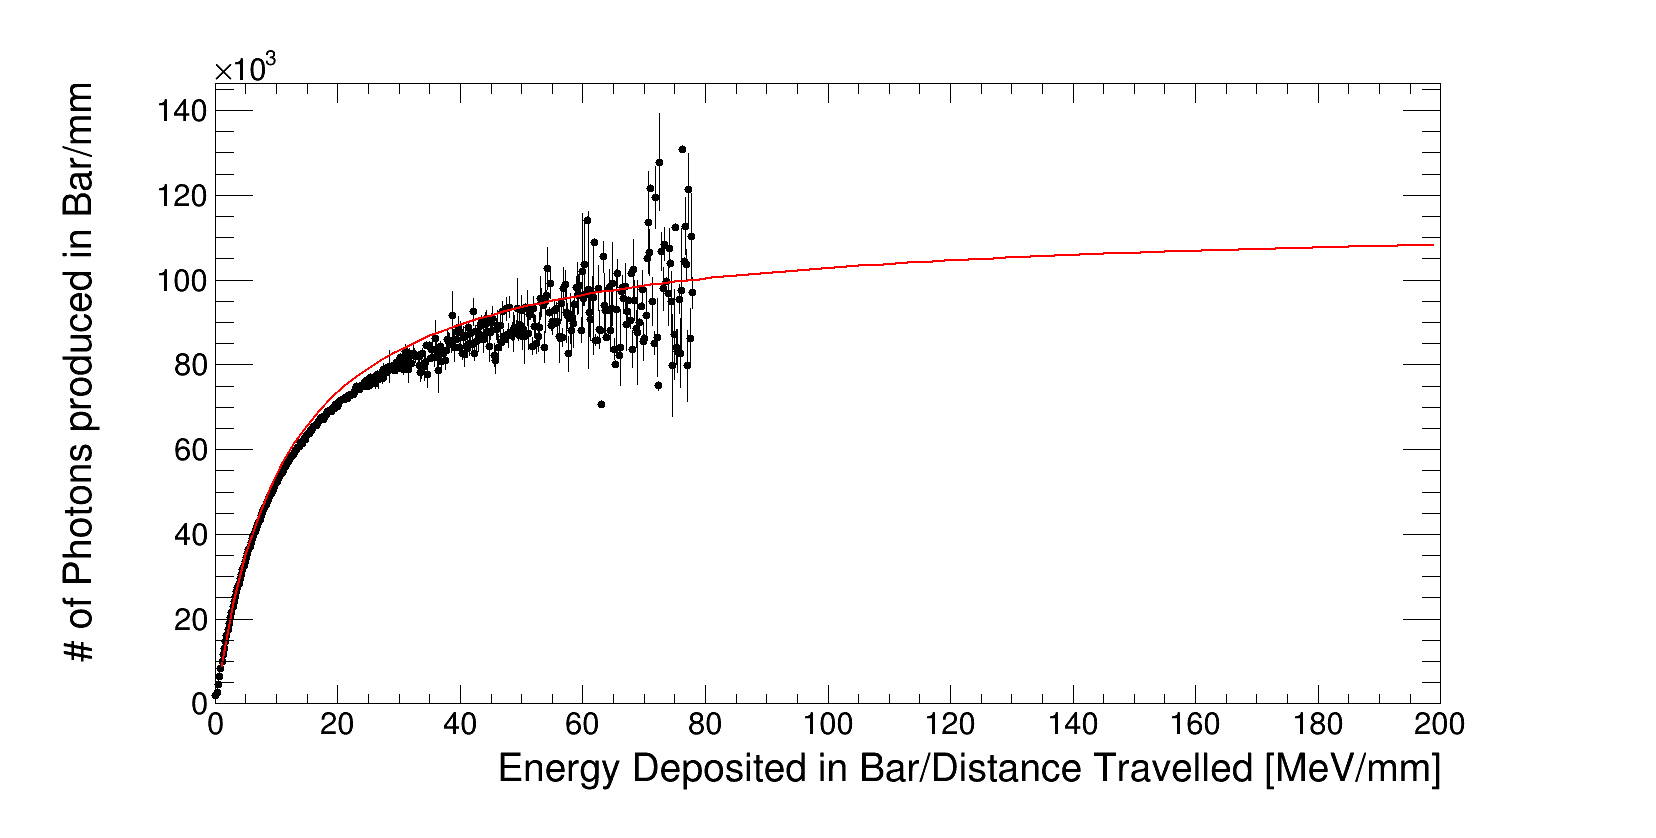
\includegraphics[width=\linewidth]{Appendix4/Figs/newDldxVsDedx/mu+_deDx_vs_dlDx.png}
 \captionof{figure}{dL/dx vs dE/dx fit using the approximation $\Delta L$/$\Delta x$ vs $\Delta E$/$\Delta x$ from the ``slice model'' simulation of scintillator for 1E6 simulated $\mu^+$ particles, $\chi^2$ = 26353.5.} 
 \label{fig:slice_AMuon_dl_dx}
\end{figure}

\begin{figure}[htbp]
 \centering
 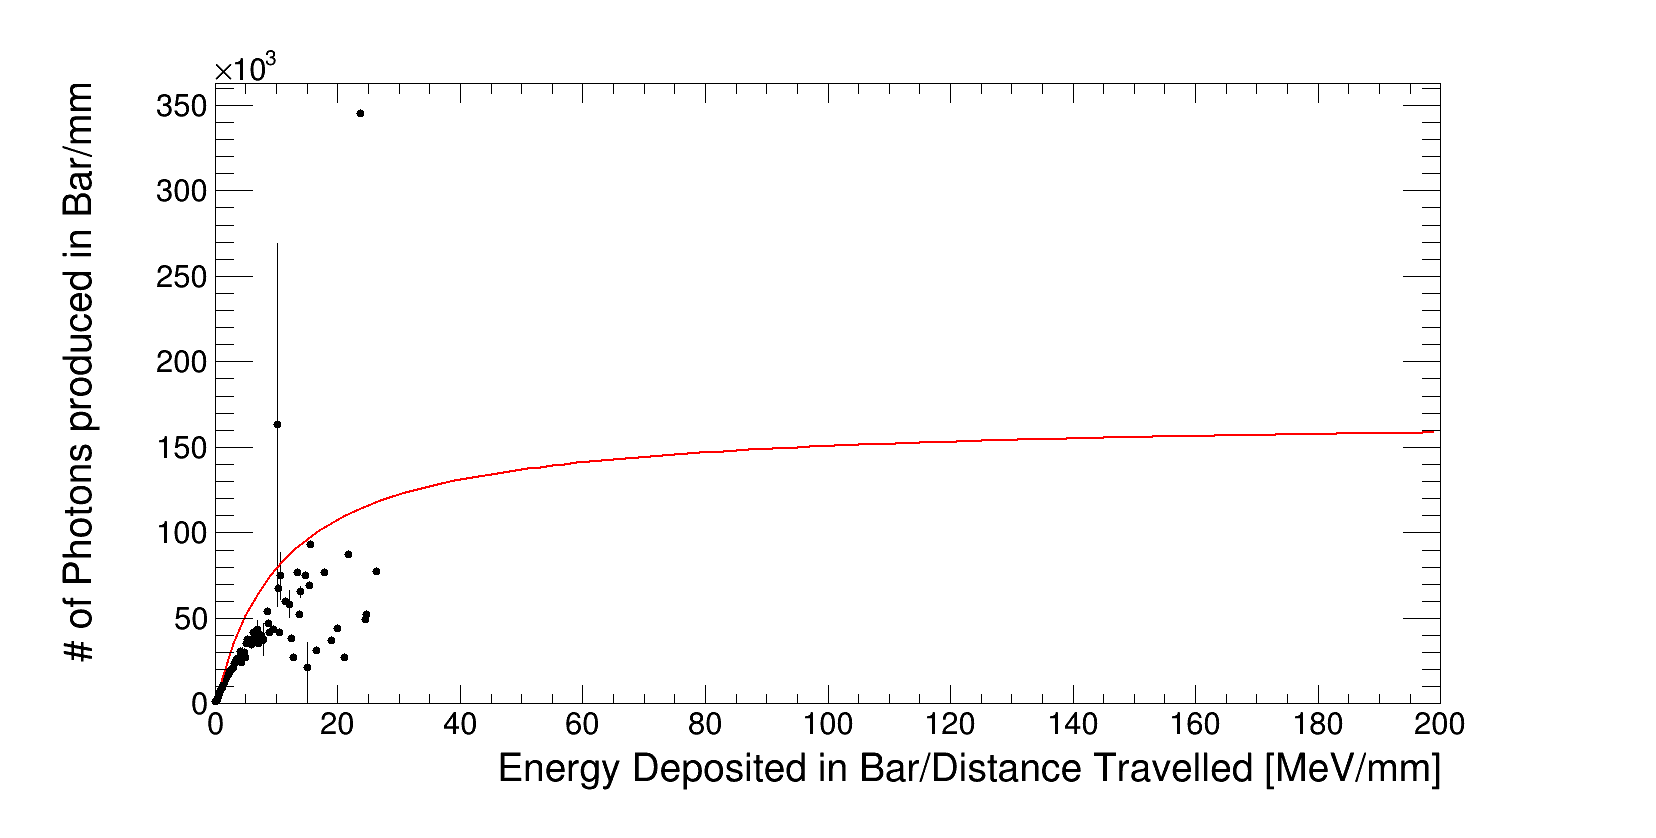
\includegraphics[width=\linewidth]{Appendix4/Figs/newDldxVsDedx/e-_deDx_vs_dlDx.png}
 \captionof{figure}{dL/dx vs dE/dx fit using the approximation $\Delta L$/$\Delta x$ vs $\Delta E$/$\Delta x$ from the ``slice model'' simulation of scintillator for 1E6 simulated $e^-$ particles, $\chi^2$ = 103856.} 
 \label{fig:slice_Electron_dl_dx}
\end{figure}

\begin{figure}[htbp]
 \centering
 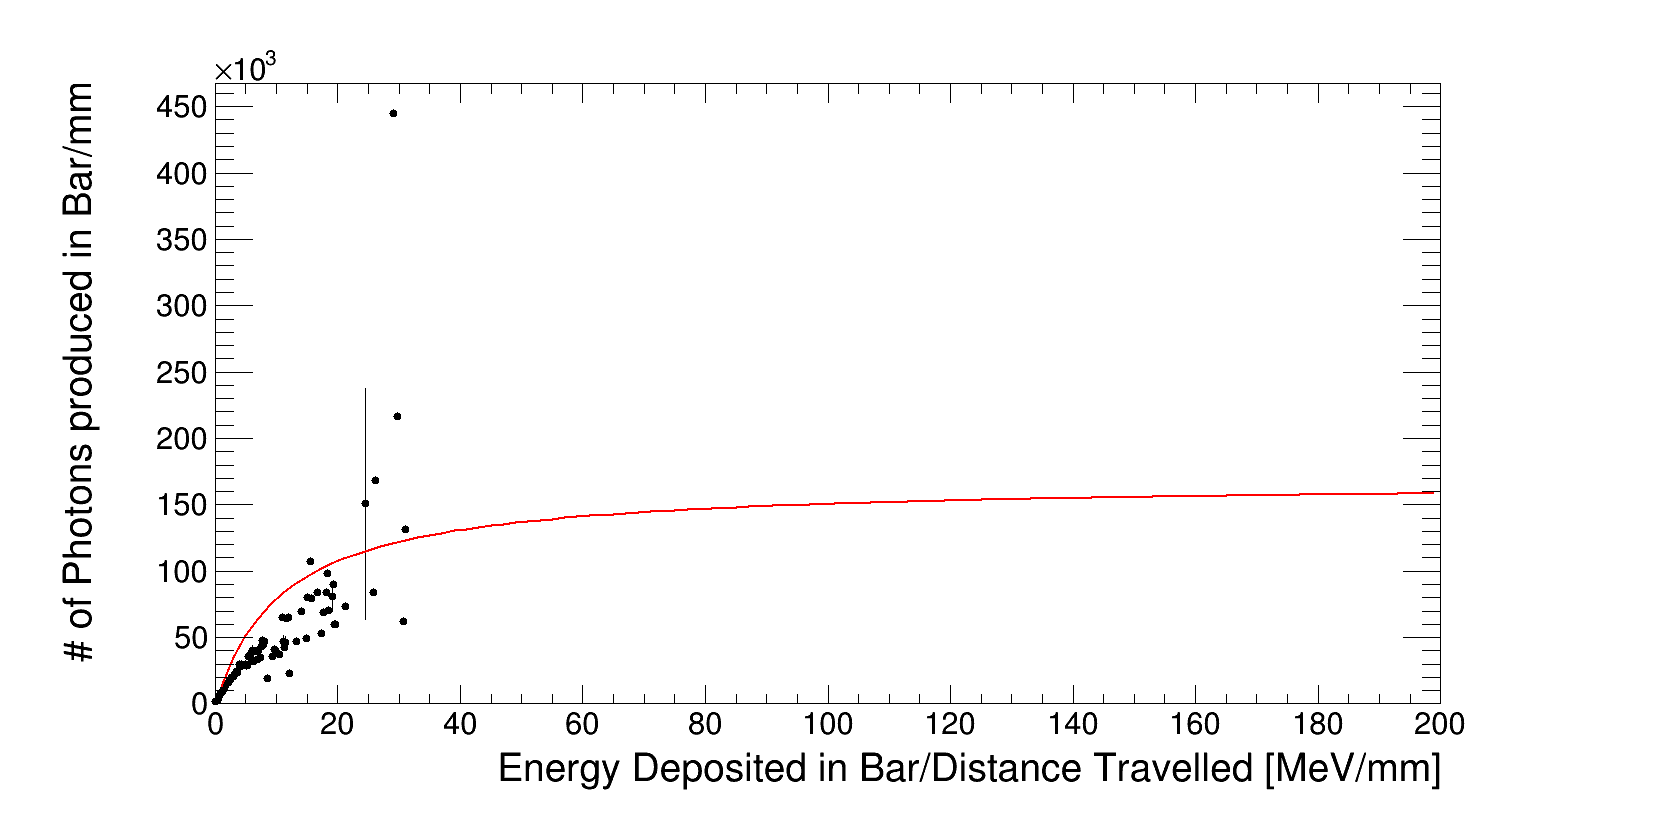
\includegraphics[width=\linewidth]{Appendix4/Figs/newDldxVsDedx/e+_deDx_vs_dlDx.png}
 \captionof{figure}{dL/dx vs dE/dx fit using the approximation $\Delta L$/$\Delta x$ vs $\Delta E$/$\Delta x$ from the ``slice model'' simulation of scintillator for 1E6 simulated $e^+$ particles, $\chi^2$ = 95343.4.} 
 \label{fig:slice_Positron_dl_dx}
\end{figure}
